%%%%%%%%%%%%%%%%%%%%%%%%%%%%%%%%%%%%%%%%%
% Beamer Presentation
% LaTeX Template
% Version 1.0 (10/11/12)
%
% This template has been downloaded from:
% http://www.LaTeXTemplates.com
%
% License:
% CC BY-NC-SA 3.0 (http://creativecommons.org/licenses/by-nc-sa/3.0/)
%
%%%%%%%%%%%%%%%%%%%%%%%%%%%%%%%%%%%%%%%%%

%----------------------------------------------------------------------------------------
%	PACKAGES AND THEMES
%----------------------------------------------------------------------------------------

\documentclass{beamer}

\mode<presentation> {

% The Beamer class comes with a number of default slide themes
% which change the colors and layouts of slides. Below this is a list
% of all the themes, uncomment each in turn to see what they look like.

\usetheme{default}
%\usetheme{AnnArbor}
%\usetheme{Antibes}
%\usetheme{Bergen}
%\usetheme{Berkeley}
%\usetheme{Berlin}
%\usetheme{Boadilla}
%\usetheme{CambridgeUS}
%\usetheme{Copenhagen}
%\usetheme{Darmstadt}
%\usetheme{Dresden}
%\usetheme{Frankfurt}
%\usetheme{Goettingen}
%\usetheme{Hannover}
%\usetheme{Ilmenau}
%\usetheme{JuanLesPins}
%\usetheme{Luebeck}
%\usetheme{Madrid}
%\usetheme{Malmoe}
%\usetheme{Marburg}
%\usetheme{Montpellier}
%\usetheme{PaloAlto}
%\usetheme{Pittsburgh}
%\usetheme{Rochester}
%\usetheme{Singapore}
%\usetheme{Szeged}
%\usetheme{Warsaw}

% As well as themes, the Beamer class has a number of color themes
% for any slide theme. Uncomment each of these in turn to see how it
% changes the colors of your current slide theme.

%\usecolortheme{albatross}
%\usecolortheme{beaver}
%\usecolortheme{beetle}
%\usecolortheme{crane}
%\usecolortheme{dolphin}
%\usecolortheme{dove}
%\usecolortheme{fly}
%\usecolortheme{lily}
%\usecolortheme{orchid}
%\usecolortheme{rose}
%\usecolortheme{seagull}
\usecolortheme{seahorse}
%\usecolortheme{whale}
%\usecolortheme{wolverine}

%\setbeamertemplate{footline} % To remove the footer line in all slides uncomment this line
\setbeamertemplate{footline}[page number] % To replace the footer line in all slides with a simple slide count uncomment this line

\setbeamertemplate{navigation symbols}{} % To remove the navigation symbols from the bottom of all slides uncomment this line
}

\usepackage{graphicx} % Allows including images
\usepackage{booktabs} % Allows the use of \toprule, \midrule and \bottomrule in tables
\usepackage{tikz}
\usetikzlibrary{arrows}
\usepackage[]{algorithm2e}
\usetikzlibrary{positioning}
%----------------------------------------------------------------------------------------
%	TITLE PAGE
%----------------------------------------------------------------------------------------

\title[Short title]{Human Mobility \\ and \\ Disease Spread Simulation} % The short title appears at the bottom of every slide, the full title is only on the title page

\author{Madotto Andrea} % Your name
\institute[UCLA] % Your institution as it will appear on the bottom of every slide, may be shorthand to save space
{
Hong Kong Baptist University \\ % Your institution for the title page
\medskip
\textit{M.Sc. Practicum} % Your email address
}
\date{20-05-2015} % Date, can be changed to a custom date

\begin{document}

\begin{frame}
\titlepage % Print the title page as the first slide
\end{frame}

\begin{frame}
\frametitle{Overview} % Table of contents slide, comment this block out to remove it
\tableofcontents % Throughout your presentation, if you choose to use \section{} and \subsection{} commands, these will automatically be printed on this slide as an overview of your presentation
\end{frame}

%----------------------------------------------------------------------------------------
%	PRESENTATION SLIDES
%----------------------------------------------------------------------------------------






%------------------------------------------------
\section{Introduction} % Sections can be created in order to organize your presentation into discrete blocks, all sections and subsections are automatically printed in the table of contents as an overview of the talk
%------------------------------------------------
\begin{frame}
\frametitle{Overview} % Table of contents slide, comment this block out to remove it
\tableofcontents[currentsection] % Throughout your presentation, if you choose to use \section{} and \subsection{} commands, these will automatically be printed on this slide as an overview of your presentation
\end{frame}
\begin{frame}
\frametitle{Introduction}
\begin{itemize}
\item Disease spread simulation based on SIR model 	\\ $\textbf{S}$usceptible $\textbf{I}$nfectives $\textbf{R}$ecovered
	\begin{itemize}
	\item SIR compartment model
	\item SIR on contact social networks 
	\end{itemize}
\item Human mobility
	\begin{itemize}
	\item Flight passengers
	\end{itemize}
\item Data visualizations
	\begin{itemize}
	\item Hive plot
	\item Data map
	\end{itemize}
\end{itemize}
\vspace{20pt}
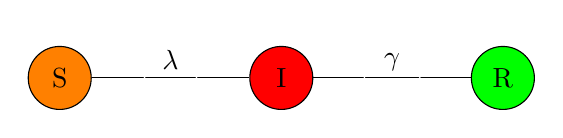
\begin{tikzpicture}[%
  every node/.style={draw,circle,minimum size=0.8cm},node distance=2cm]
  % the vertices
  \node[fill=orange] (source) {S};
  \node[fill=red,right=of source] (three) {I};
  \node[fill=green,right=of three] (six) {R};
  % the edges
  \draw (source) -- (three) node [midway,above=-5pt, fill=none,draw=white] {$\lambda$} -- (six)node [midway,above=-6pt, fill=none,draw=white]{$\gamma$} ;
\end{tikzpicture}
\end{frame}


%------------------------------------------------
\section{SIR Models}


\subsection{Compartment model}


\begin{frame}
\frametitle{Overview} % Table of contents slide, comment this block out to remove it
\tableofcontents[currentsection] % Throughout your presentation, if you choose to use \section{} and \subsection{} commands, these will automatically be printed on this slide as an overview of your presentation
\end{frame}
%------------------------------------------------

\begin{frame}
\frametitle{SIR: Compartment model}
\begin{columns}[c] % The "c" option specifies centered vertical alignment while the "t" option is used for top vertical alignment

\column{.45\textwidth} % Left column and width

\begin{itemize}
\item System of differential equations to simulate the disease propagations
\item Three different variables (S,I and R) that represents the status of each compartment
\item Where $\beta$ represent the disease transmission rate
\item Where $\gamma$ describes the recovery rate
\end{itemize}


\column{.5\textwidth} % Right column and width
\begin{equation}
\frac{\textit{d}S}{\textit{dt}} =-\lambda \cdot S \nonumber
\end{equation}

\begin{equation}
\frac{\textit{d}I}{\textit{dt}} =\lambda \cdot S - \gamma \cdot I \nonumber
\end{equation}

\begin{equation}
\frac{\textit{d}R}{\textit{dt}} =\gamma \cdot I \nonumber
\end{equation}

\begin{equation}
\lambda= \beta \cdot \frac{I}{N} \nonumber
\end{equation} 

\end{columns}
\end{frame}

%------------------------------------------------

\begin{frame}
\frametitle{Compartment model: $R_0$}

Another important parameter, called basic reproduction number, is given by:
\begin{equation}
R_0=\frac{\beta}{\lambda} \nonumber
\end{equation}
and it has well known value, useful to have a correct parametrization.

\begin{table}[H]
\begin{tabular}{|l|l|c|}
\hline
\multicolumn{1}{|c|}{\textbf{Disease}} & \multicolumn{1}{c|}{\textbf{Transmission}} & \textbf{$R_0$} \\ \hline
Diphtheria                             & Saliva                                     & 6-7         \\ \hline
Smallpox                               & Airborne droplet                           & 5-7         \\ \hline
Mumps                                  & Airborne droplet                           & 4-7         \\ \hline
HIV/AIDS                               & Sexual contact                             & 2-5         \\ \hline
SARS                                   & Airborne droplet                           & 2-5         \\ \hline
Influenza(1918 pandemic strain)        & Airborne droplet                           & 2-3         \\ \hline
Ebola(2014 Ebola outbreak)             & Bodily fluids                              & 1.5-2.5     \\ \hline
\end{tabular}
\caption{Values of $R_0$ of well-known infectious diseases}
\end{table}
\end{frame}

%------------------------------------------------

\begin{frame}
\frametitle{Compartment model: implementation and result}
\begin{columns}[c] % The "c" option specifies centered vertical alignment while the "t" option is used for top vertical alignment

\column{.45\textwidth} % Left column and width

\begin{itemize}
\item Python with scipy and numpy library
\item Implement of the Algorithm 1
\item Basic setting: $S=100000$, $I=3$, $R=0$, $\beta=0.5$, $\gamma=0.112$ and $t=100$
\end{itemize}


\column{.5\textwidth} % Right column and width
\begin{algorithm}[H]\label{alg:alg2}
 \KwData{Set of parameters: \{S,I,R,N,$\gamma$,$\beta$\}}
 \KwResult{Result statistic of the simulation}
 SetParameters(S,I,R,N,$\lambda$,$\beta$)\;
 \ForEach{$t\in T$}{
	S($t$)=$-\beta \cdot \frac{I}{N} \cdot S(t-1)$\;
	I($t$)=$\beta \cdot \frac{I}{N} \cdot S(t-1) - \gamma \cdot I(t-1) $\;
	R($t$)=$\gamma \cdot I(t-1)$\;
 }
\caption{Pseudocode of compartmental model simulation}
\end{algorithm}
\end{columns}


\end{frame}

%------------------------------------------------

\begin{frame}
\frametitle{Compartment model: implementation and result (cont)}
\begin{figure}[H]\label{fig:sir}
\centering	
\includegraphics[scale=0.4]{img/Sir_comp.png}
\caption{SIR compartment simulation with $R_0=4$}
\end{figure} 

\end{frame}


\subsection{Social Contact Networks}


\begin{frame}
\frametitle{Overview} % Table of contents slide, comment this block out to remove it
\tableofcontents[currentsection] % Throughout your presentation, if you choose to use \section{} and \subsection{} commands, these will automatically be printed on this slide as an overview of your presentation
\end{frame}
%------------------------------------------------
\begin{frame}
\frametitle{SIR: Social Contact Networks}
\begin{itemize}
\item Weighted graph $G(V,E)$ describe a contact social network
\item $V=\{v_1,...,v_n\}$ a set of nodes that represents the different individuals
\item Set of label $L$ in the node for representing the state of the nodes (S,I or R)
\item $E=\{e_1,...,e_n\}\subseteq (V \times V)$ a list of edges that represent the connection between different individuals
\item Each edge $e=(v_i,v_j)$ is weighted by the duration of the contact between $v_i$ and $v_j$
\item Probability of infection (depend on the status of the node, the state of its neighbour and the duration of the contact) 
\end{itemize}
\begin{equation}
w_i=\sum_{e\in adj_I(v_i)} l_e \qquad l_e \in duration(e)  \nonumber
\end{equation} 
\begin{equation}
p(v_i)=1-(1-r)^{w_i}
\end{equation}
\end{frame}


%------------------------------------------------
\begin{frame}
\frametitle{SIR: Social Contact Networks}
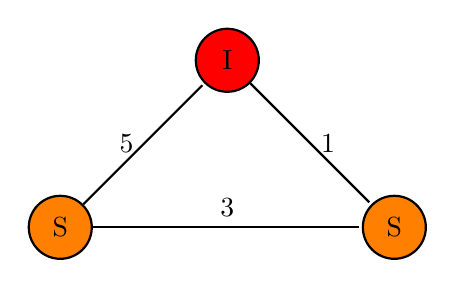
\begin{tikzpicture}[-,>=stealth',shorten >=1pt,auto,node distance=3cm,
                    thick,main node/.style={circle,draw,minimum size=0.8cm}]

  \node[main node,fill=red] (1) {I};
  \node[main node,fill=orange] (2) [below left of=1] {S};
  \node[main node,fill=orange] (4) [below right of=1] {S};

  \path[]
    (1) edge node [right] {1} (4)
    (2) edge node [left] {5} (1)
        edge node {3} (4)
;
\end{tikzpicture}
\vspace{10pt}
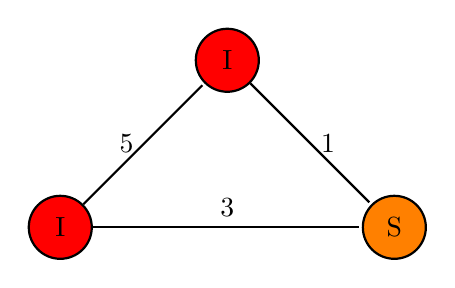
\begin{tikzpicture}[-,>=stealth',shorten >=1pt,auto,node distance=3cm,
                    thick,main node/.style={circle,draw,minimum size=0.8cm}]

  \node[main node,fill=red] (1) {I};
  \node[main node,fill=red] (2) [below left of=1] {I};
  \node[main node,fill=orange] (4) [below right of=1] {S};

  \path[]
    (1) edge node [right] {1} (4)
    (2) edge node [left] {5} (1)
        edge node {3} (4)
;
\end{tikzpicture}
\vspace{10pt}
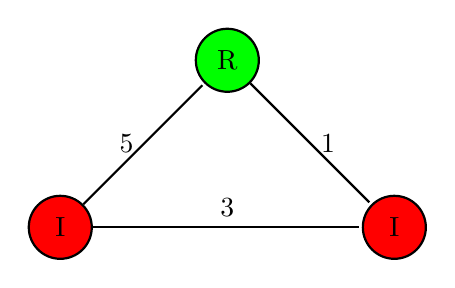
\begin{tikzpicture}[-,>=stealth',shorten >=1pt,auto,node distance=3cm,
                    thick,main node/.style={circle,draw,minimum size=0.8cm}]

  \node[main node,fill=green] (1) {R};
  \node[main node,fill=red] (2) [below left of=1] {I};
  \node[main node,fill=red] (4) [below right of=1] {I};

  \path[]
    (1) edge node [right] {1} (4)
    (2) edge node [left] {5} (1)
        edge node {3} (4)
;
\end{tikzpicture}
\vspace{10pt}
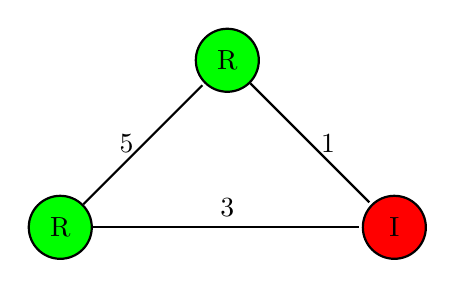
\begin{tikzpicture}[-,>=stealth',shorten >=1pt,auto,node distance=3cm,
                    thick,main node/.style={circle,draw,minimum size=0.8cm}]

  \node[main node,fill=green] (1) {R};
  \node[main node,fill=green] (2) [below left of=1] {R};
  \node[main node,fill=red] (4) [below right of=1] {I};

  \path[]
    (1) edge node [right] {1} (4)
    (2) edge node [left] {5} (1)
        edge node {3} (4)
;
\end{tikzpicture}
\vspace{-30pt}
\begin{figure}
\caption{Example with 3 nodes, 3 edges and $\Delta_{t_I}=2$}
\end{figure}

\end{frame}
%------------------------------------------------

\begin{frame}[shrink=28]
\frametitle{Social Contact Networks: details and implementation}
\begin{columns}[c] % The "c" option specifies centered vertical alignment while the "t" option is used for top vertical alignment

\column{.45\textwidth} % Left column and width

\begin{itemize}
\item Graph database to implement the network (Neo4j)
\item Py2neo library to connect Python to the database 
\item Implementation of the Algorithm 2 with Python	
\end{itemize}
\vspace{10pt}
\begin{itemize}
\item A node can remain infect for a $\Delta_{t_I}$ period
\item calculateProbInfect($v_i$) use the Equation 1
\item graphUpdate(V) update all the labels just after the finish of the For
\end{itemize}
\vspace{10pt}

\begin{itemize}
\item Note that a susceptible node can become infected just if it has at least one infected node
\item $\Delta_{t_I}$ represent the infection duration, after this time the node become recovered

\end{itemize}

\column{.3\textwidth} % Right column and width

\begin{algorithm}[H]\label{alg:alg2}
 \KwData{Social network graph}
 \KwResult{Statistic on the simulation and effectiveness of the tested intervention}
 graphCreate()\;
 \ForEach{$t\in T$}{
 applyIntervention($G$)\;
  \ForEach{$v_i \in V$}{
  $p_i$=calculateProbInfect($v_i$)\;
  $r_i$=random(0,1)\;
  \If{$r_i \geq p_i$}{
   $v_i.status$=INFECTED\;
   }
 }
 graphUpdate(V)\;
 }
\caption{Pseudocode of simulation}
\end{algorithm}

\end{columns}

\end{frame}


%------------------------------------------------

\begin{frame}
\frametitle{Social Contact Networks: Technologies}
\begin{itemize}
\item Neo4j: ensures the atomicity, consistency, isolation and durability during the graph manipulations. In addiction, it provides flexibility, scalability and high performance.
\begin{figure}[H]
\raggedright
\includegraphics[scale=0.25]{img/neo4j-logo-2015.png}
\end{figure} 
\item Py2neo: is a client library and comprehensive toolkit for working with Neo4j from within Python applications and from the command line. The core library has no external dependencies and has been carefully designed to be easy and intuitive to use.
\begin{figure}[H]
\raggedright
\includegraphics[scale=0.2]{img/py2neo.png}
\end{figure} 
\end{itemize} 

\end{frame}


%------------------------------------------------
\section{Datasets}

\begin{frame}
\frametitle{Overview} % Table of contents slide, comment this block out to remove it
\tableofcontents[currentsection] % Throughout your presentation, if you choose to use \section{} and \subsection{} commands, these will automatically be printed on this slide as an overview of your presentation
\end{frame}

\begin{frame}
\frametitle{Datasets: Scientific collaboration networks}
\begin{itemize}
\item This dataset represents the collaborations between the authors and co-authors in the scientific papers
\item Connection between two authors if they have their names in the same publication
\item Duration of the contact is represented by the number of the papers that the two authors have in common
\item The authors spend time, during the days, with the co-authors and the duration of the contact is proportional to the number of the papers they work together
\end{itemize}
\end{frame}
%------------------------------------------------

\begin{frame}
\frametitle{Datasets: Student from University of California}
\begin{itemize}
\item Represents the relationships between the students in the University of California
\item Connection between the students if they exchange messages
\item exchange a lot of message, then they have higher contact duration
\item We consider the duration of the contact as proportional to the number of the message exchanged between the students
\end{itemize}
\end{frame}
%------------------------------------------------

\begin{frame}
\frametitle{Datasets: Summary}
\begin{table}[H] \label{Tab:1}
\centering
\resizebox{\columnwidth}{!}{%
\begin{tabular}{|l|l|l|l|}
\hline
\textbf{Dataset name}                 & \textbf{Number of nodes} & \textbf{Number of edge} & \textbf{Density} \\ \hline
Scientific collaboration networks     & 1589                     & 2741                    & 2.97             \\ \hline
Student from University of California & 1899                     & 8695                    & 20.97            \\ \hline
\end{tabular}
}
\caption{Summary of the datasets}
\end{table}

Note that, this dataset comes from previous article and web repository. Hence, before import this data to Neo4j we have clean and sometimes summarized. To do that, we imported all the data in MySQL.
\end{frame}
\section{Infection, vaccination and result}

\begin{frame}
\frametitle{Overview} % Table of contents slide, comment this block out to remove it
\tableofcontents[currentsection] % Throughout your presentation, if you choose to use \section{} and \subsection{} commands, these will automatically be printed on this slide as an overview of your presentation
\end{frame}
%------------------------------------------------

\begin{frame}
\frametitle{Experiment: infections}
First of all, we run the simulation in all the datasets using the Algorithm 2. This because we need to have a referent measurements in order to classify the countermeasure effectiveness. \\
For reference we show the result of the Scientific collaboration network. The basic setting are: $r=0.05$ and $t=20$.

\begin{figure}[H]\label{fig:scie_sir}
\centering	
\includegraphics[scale=0.4]{img/Scientific_basic.png}
\caption{Scientific collaboration networks, basic simulation}
\end{figure} 

\end{frame}
%------------------------------------------------

\begin{frame}
\frametitle{Experiment: vaccinations}
\begin{itemize}
\item To contain the spread of the virus
\item The application of vaccine shot to the network will start after the ratio $I/S$ is grater 0.1
\item The effectiveness of the vaccination is not 100\% but just 70-80\% 
\item We would like to represent the vaccination decision making of an single node in the network.
	\begin{itemize}
	\item Depending on the cost of the vaccination 
	\item Depending on the behaviours of the neighbour
	\end{itemize}
\end{itemize}



\end{frame}
%------------------------------------------------


\begin{frame}
\frametitle{Vaccinations decision making}
To model the decision making we implement the following formula
\begin{equation}\label{equa:lamb}
\lambda_i=\frac{N_i^{non}}{( N_i^{non} + N_i^{vac})} \nonumber
\end{equation}      
\begin{equation} \label{equa:r}
r=\frac{c_{vac}}{c_{inf}} \nonumber
\end{equation} 
where $i$ is an index of a node in the network, $c_{vac}$ represent the cost of the vaccination and $c_{inf}$ the costs of disease infection. The number $r$ is called reproduction number and more smaller means cheaper. Then a node take the vaccine if 
\begin{equation}
\begin{cases} 
r< \lambda_i \qquad take \ the \ vaccine \\ r \geq \lambda_i \qquad don't \ take \ the \ vaccine
\end{cases}
\end{equation}
\end{frame}

%------------------------------------------------


\begin{frame}
\frametitle{Vaccinations result}
\begin{figure}[H]\label{fig:perc_vac}
\centering	
\includegraphics[scale=0.6]{img/vaccScientfic.png}
\caption{Percentage of vaccinated people and their reproduction number on the Scientific collaboration network dataset}
\end{figure} 

\end{frame}
%------------------------------------------------


\begin{frame}
\frametitle{Vaccinations result (cont)}
\begin{figure}[H]\label{fig:perc_diff}
\raggedright
\includegraphics[scale=0.55]{img/Scientific_diff_perc.png}
\caption{Percentage difference infected and vaccinated on the Scientific collaboration network dataset}
\end{figure} 

\end{frame}
%------------------------------------------------

\begin{frame}
\frametitle{Vaccinations result (cont)}
\begin{figure}[H]\label{fig:perc_diff}
\centering	
\includegraphics[scale=0.35]{img/graphtotal_science.png}
\caption{Plot of four run with different $r$ on the Scientific collaboration network dataset}
\end{figure}

\end{frame}

\section{Hive Plot}
\begin{frame}
\frametitle{Overview} % Table of contents slide, comment this block out to remove it
\tableofcontents[currentsection] % Throughout your presentation, if you choose to use \section{} and \subsection{} commands, these will automatically be printed on this slide as an overview of your presentation
\end{frame}
%------------------------------------------------

\begin{frame}
\frametitle{Why use Hive Plot and what is an Hive Plot}
\begin{block}{Why?}
The network graphs in the datasets have a lot of nodes and edges, thus it is easy to have the hairball effect when we plot the entire graph in just one figure. The following picture is just a network with 300 nodes and 600 edges.
\end{block}
\begin{figure}[H]\label{fig:perc_diff}
\centering	
\includegraphics[scale=0.30]{img/graph4.PNG}
\end{figure}

\end{frame}
%------------------------------------------------


\begin{frame}
\frametitle{Why use Hive Plot and what is an Hive Plot (Cont)}
\begin{block}{What is an Hive Plot?}
This visualization fixes the position of each node among three or more different axis and plots only the useful edges.
\end{block}
\begin{figure}[H]\label{fig:perc_diff}
\centering	
\includegraphics[scale=0.30]{img/hive.PNG}
\end{figure}

\end{frame}

%------------------------------------------------


\begin{frame}
\frametitle{Hive plot in SIR model}
\begin{itemize}
\item Not show the edge between the node which have the same label
\item Be able to sort the nodes in some ways (e.g. sort by age, degree of outgoing edges)
\item The orange nodes represents susceptible individuals (in the S axis)
\item The red nodes represents infected one (in the I axis)
\item The green represents recovered (in the R axis)
\item The purple represents vaccinated (in the V axis)
\end{itemize}
We have create two type of visualization: one represent the current state of the graph and another one represent the evolution of the graph. This means show which nodes pass between different status.
\end{frame}

%------------------------------------------------

\begin{frame}
\frametitle{Hive plot SIR model: current state}
\begin{figure}[H]\label{fig:perc_diff}
\centering	
\includegraphics[scale=0.45]{img/hive1.PNG}
\vspace{20pt}
\includegraphics[scale=0.405]{img/dataset1.PNG}
\caption{Current state of the graph. The hive on the left is the day 0 and the right the day 5}
\end{figure}
\end{frame}

%------------------------------------------------

\begin{frame}
\frametitle{Hive plot SIR model: evolution of the graph}
\begin{figure}[H]\label{fig:perc_diff}
\centering	
\includegraphics[scale=0.45]{img/vacc.PNG}

\caption{Represent the transaction between the node during the simulation}
\end{figure}
\end{frame}

%------------------------------------------------

\begin{frame}
\frametitle{Hive plot SIR model: Final result}
\begin{figure}[H]\label{fig:perc_diff}
\centering	
\includegraphics[scale=0.1]{img/tot_vacc.jpg}
\vspace{10pt}
\includegraphics[scale=0.1185]{img/tot_hive.jpg}

\end{figure}
\end{frame}
%------------------------------------------------
\section{Human mobility}
\begin{frame}
\frametitle{Overview} % Table of contents slide, comment this block out to remove it
\tableofcontents[currentsection] % Throughout your presentation, if you choose to use \section{} and \subsection{} commands, these will automatically be printed on this slide as an overview of your presentation
\end{frame}
%------------------------------------------------

\begin{frame}
\frametitle{Human mobility}
\begin{itemize}
\item The human mobility is an important aspect in the world disease transmission
\item Analyze this aspect through a flight travel simulation
\end{itemize}
\vspace{10pt}
We have two different layer of simulation:
\begin{itemize}
\item Passenger between the country, that is the flight network. Then, we use the Algorithm 2 (SIR Social contact network)
\item Inside every country. Then, we use the Algorithm 1 (SIR compartment model)
\end{itemize}
Therefore we have 200 node (country) in the graph, and for each country we run the compartment model simulation. 
\end{frame}



%------------------------------------------------

\begin{frame}
\frametitle{Human mobility: datasets}
We combine three different datasets:
\begin{itemize}
\item Open flight, here we take all the information regarding the airport, such us: Name, City, Country, IATA/FAA, Longitude and Latitude
\item Vbd-air, here we found information about the number of passengers for each route
\item CIA, coordinate of the center of every country.
\end{itemize} 
To combine this information we used Mysql and Python. The first to join different table, and the second to standardize and clean the data. \\
Just after this process we import that in Neo4j for the simulation.
\end{frame}
%------------------------------------------------


\begin{frame}
\frametitle{Human mobility: implementation}
\begin{itemize}
\item Use Neo4j for the network simulation
\item Each node maintain three variable S,I and R
\item Compartment simulation in each node
\item Global clock
\end{itemize}
\begin{figure}[H]\label{fig:perc_diff}
\centering	
\includegraphics[scale=0.6]{img/flight.jpeg}
\end{figure}

\end{frame}
%------------------------------------------------

\begin{frame}
\frametitle{Human mobility: data visualization}
To visualize the flight network and the disease propagation we use an info graphic map. 
\begin{itemize}
\item D3js map framework
\item Display a flat map and a globe map to better visualize the map
\item Orange for the susceptible countries
\item Dark orange for countries with at least $15\%$ of the population is infected
\item Red for countries with at least $50\%$ of the population is infected
\item Green for countries with at least $50\%$ of the population is recovered
\end{itemize} 


\end{frame}
%------------------------------------------------

\begin{frame}
\frametitle{Human mobility: data visualization (cont)}
\begin{figure}[H]\label{fig:perc_diff}
\centering	
\includegraphics[scale=0.09]{img/tot_map1.jpg}
\vspace{10pt}
\includegraphics[scale=0.09]{img/tot_map2.jpg}

\end{figure}


\end{frame}
%------------------------------------------------
\section{Conclusion}
\begin{frame}
\frametitle{Overview} % Table of contents slide, comment this block out to remove it
\tableofcontents[currentsection] % Throughout your presentation, if you choose to use \section{} and \subsection{} commands, these will automatically be printed on this slide as an overview of your presentation
\end{frame}
%------------------------------------------------


\begin{frame}
\frametitle{Conclusion}
\begin{itemize}
\item We have analysed two different techniques to simulate the infection process
\begin{itemize}
\item based on a social contact network 
\item based on a compartment model
\end{itemize}
\item We saw how the decision of an individual, depending on the cost of the vaccination and the neighbours' decision, influences the spread of the disease
\item How human movement by flight influence the propagation of a virus
\item we implement two methods to display the result in clear and understandable way
\begin{itemize}
\item hive plot
\item info graphic map
\end{itemize}
\end{itemize}
\end{frame}

%----------------------------------------------------------------------------------------


\begin{frame}
\Huge{\centerline{Q \& A}}
\end{frame}

%----------------------------------------------------------------------------------------

\end{document} 